\section{Depth-Based Tiebreaking for A*}

\label{sec:depth}

In Zerocost domains, the search space has a lot of zero-cost edges,
producing a large final plateau $\plateau{f^*,0}$. In a final plateau,
all nodes have $h=0$ which inhibit the $h$-based tiebreaking to provide
a useful guidance toward a goal. Without adequate measure, search
algorithms may fail to keep track of the current search progress.

The \emph{depth} of a node is an instance of such measurement.  It is an
integer value representing the distance (number of steps) from the
\emph{entrance} of the plateau.  An \emph{entrance} of the plateau is
the first node which entered the plateau, along the path from the
initial node. These notions are depicted in
\refig{fig:plateau-depiction}. It is equivalent to the $g$-value which is
restricted to a particular plateau and is assuming the unit cost edges.

\begin{figure}[htbp]
  \centering
  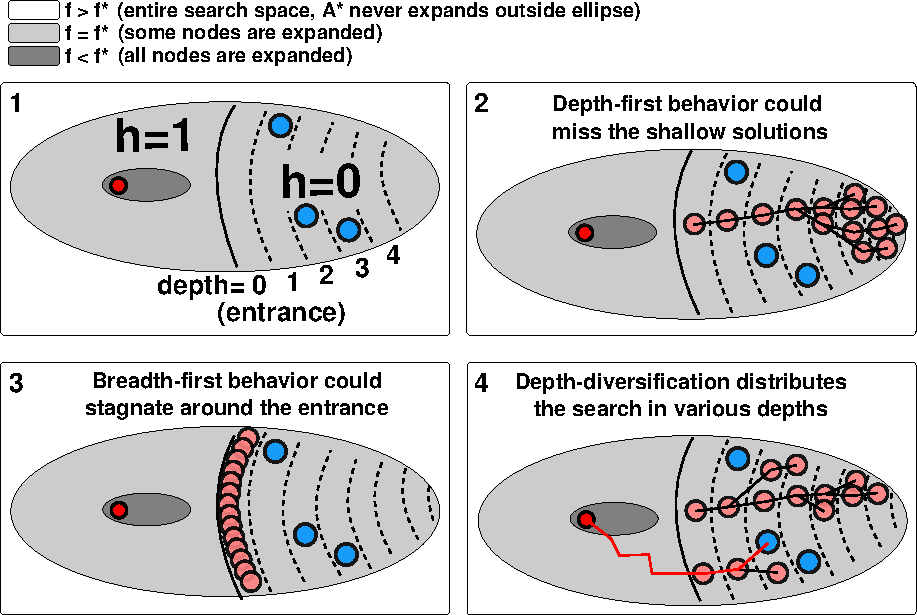
\includegraphics{img/astar/plateau-2.pdf}
 \caption{The nodes in a plateau are divided into several layers, and each layer have the corresponding depth. Since all nodes have $f=f^*$, depth does not affect optimality. The goals in both shallower or deeper region yield cost-optimal solutions.
 }
 \label{fig:plateau-depiction}
\end{figure}

The depth $d(n)$ of a
node $n$ is 0 when $n$ and the parent node $m$ have the different key
values for a sorting strategy, and $d(n)=d(m)+1$ when they have the same
key values: For example, in \astar with $h$-based tiebreaking, the key
values of a node are represented as a vector $[f,h]$, and they are same
when they are pairwise equivalent (i.e. $f(n) = f(m) \land h(n) =
h(m)$).  Having the same key values means that $n$ and $m$ are in the
same plateau. \todo{Figure}

The traditional \lifo and \fifo tiebreaking strategy are
searching the plateau region in a decreasing or increasing order of the depth.
\lifo strategy always selects the most recently generated node
within $\plateau{f,h}$, and the behavior in the plateau is equivalent to depth-first search.
Thus, it results in always selecting the largest depth
buckets as depicted in \refig{fig:plateau-depiction} (left).
Similarly, the behavior of \fifo strategy 
in a plateau is equivalent to breadth-first search. Thus \fifo strategy
always selects the nodes with least depth (right).
Note that therefore $[f,h,\lifo]$ is equivalent to $[f,h,-d,\lifo]$ and
$[f,h,\fifo]$ is equivalent to $[f,h,d,\fifo]$.

\begin{figure}[htbp]
 \centering
  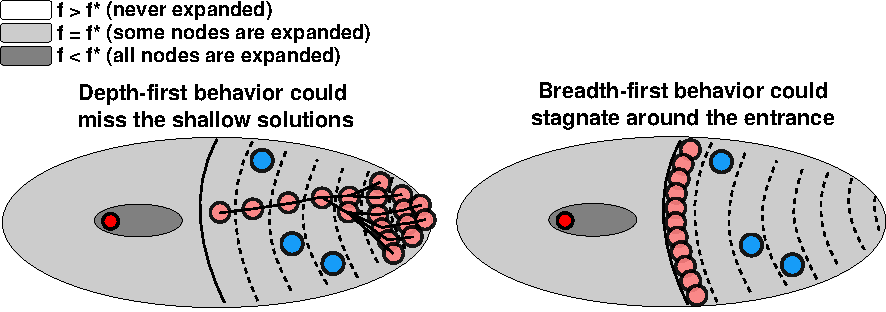
\includegraphics{img/astar/plateau-3.pdf}
 \caption{(\textbf{Left}) \lifo tiebreaking strategy implies a depth-first behavior in a
 plateau, which could miss the solution concentrated near the entrance.
 (\textbf{Right}) \fifo tiebreaking strategy implies a breadth-first behavior in a
 plateau, which could fail to reach a solution in the deeper region
 within the time limit.}
 \label{fig:plateau-depiction}
\end{figure}

The problem in these traditional strategies is that we have no knowledge
on whether the goals are located near or far from the entrance. Remind
that since $f=f^*$, any goals in this plateau are optimal
regardless of the depth: A goal node in a shallower region or a deeper
region both yields a cost-optimal solution. However, until we find a
solution, we do not know how the goals are distributed among various
depths. In some problem instance the goals can be concentrated around
the entrance, and in another problem instance the goals can be
concentrated in some large depth $k$.

% \begin{figure}[htbp]
%  \includegraphics{img/astar/final-plateau4-2.png}
%  \label{fig:plateau-depiction-all-optimal}
% \end{figure}

The best-first search (\fifo), which naturally focuses the search around
the entrance favoring the smaller depths, should perform better in the
former case, while it also severely degrade the performance in the
latter case because it searches the
shallower region exhaustively and takes too much time to reach the depth
where the goals exist.
Exactly the opposite could happen to depth-first search (\lifo):
\lifo greedily explores the
plateau region and may find a solution in the deeper region quickly but
could also miss the solution in the shallower region.
Thus, both \fifo and \lifo tiebreaking have pathological behaviors.

By an adversary argument, we propose a depth-based \emph{diversification}
tiebreaking strategy, which diversify the search among various depths.
Its search behavior is not biased toward any particular direction and
does not exhibit the pathological behavior.

In this strategy, the nodes are inserted into buckets
associated with depths, and upon expansion, search effort is distributed
among various depths. Notice that it does not ``sort'' the nodes
according to the increasing or decreasing order of depth,
and instead ``diversify'' the node expansion
within the plateau. We mark such a diversification family of
tiebreaking strategies by enclosing it in brackets such as $[f,h,\depth]$.

In order to diversify the expansion among depths, we propose simply
iterating over the depth buckets. There is a counter $d_c$ initialized
to 0, which stores the depth which was selected in the last expansion.
In each expansion, it decrements the counter ($d_c\leftarrow d_c-1$) and
expands from the bucket of $d_c$. When $d_c$ reaches below 0, then $d_c$
is reset to the current largest depth in the plateau.
It is possible to adopt a
non-deterministic, randomized selection, as we have done in a conference
version of this paper, however we eliminate the possibility of the
results being affected by random seeds. It also makes a theoretical
analysis more convenient in the later section.

\begin{figure}[htbp]
 \centering
  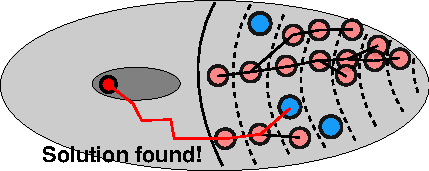
\includegraphics{img/astar/plateau-4.pdf}
 \caption{Depth-based diversification allows \astar to search the plateau space
 uniformly and sparsely, avoiding the concentration to shallower depths, while
 suppressing the excessive exploration to the deeper region. This
 balances the exploration and exploitation.}
 \label{fig:plateau-depiction-all-optimal}
\end{figure}

% We later show that
% \fifo and \lifo strategies are incomplete when the size of the plateau
% region is inifinite, while our \id is probabilistically complete.

\subsection{The Scope Captured by Depth-Based Tiebreaking}

Depth-based tiebreaking has no effect when the key values for measuring
the depth are always updated and thus all nodes have depth 0. A key
value is a single $f$ when $h$-based tiebreaking is not present, and a
pair of $f$ and $h$ when $h$-based tiebreaking is present. When all
nodes have depth 0, the search is equivalent to the case where 
the depth-based strategy is not present.
% 
This happens when the target problem contains
positive costs\footnote{not to be confused with non-negative cost} only.
Let a node $n$ is reached from a node $m$. Assume
 $g(n)>g(m)+c$ where $c$ is a positive edge cost, and the parent of $n$
 is updated to $m$.

\begin{itemize}
 \item 
       If $f(n)=f(m)$, $h(n)<h(m)$ should hold because the new value of
       $g(n)$ is $g(m)+c>g(m)$. Therefore the depth is 0.
 \item If $h$-value is unchanged and $g$ is increased due to a positive
       cost edge, then $f$ is also increased, thus the depth is 0.
\end{itemize}

One might wonder what if the evaluated nodes are already visited from
another parent (old parent) with smaller $g$ value, and the new $g$ value does not change it,
which may cause the new parent and the child node may have the same $f$ and
same $h$. It does not result in a positive depth because it does not update the parent. The depth of a
child remains the old value (using the old parent), which is 0.


\subsection{Tiebreaking within Depth Buckets}

Since there can be still multiple nodes within the same depth bucket, a
default tiebreaking is still necessary to break ties among them.
We can, for example, apply \lifo, \fifo or \ro (random order) policies
at this level.

There could be still a room for heuristic-agnostic improvements at
this level, while this is not in the scope of this paper.
For example, while depth metric measures and diversifies the depth in a plateau,
other techniques can non-trivially diversify the search in a breadth direction.
Such techniques may include pruning techniques such as 
Symmetry Breaking \cite{Fox1998,pochter2011exploiting,domshlak2013symmetry}
or Partial Order Reduction \cite{hall2013faster,wehrle2013relative}.

While these methods are most often described as ``pruning techniques'',
it can be rephrased as ``removing the cardinality bias to particular set
of nodes which share the same characteristics'' because they both aim to
prune the redundant nodes. Note that redundancy causes a biased 
search effort. For example, imagine we have a
set of nodes $S=\{a_1, a_2, a_3, a_4, b, c, d\}$ where
$A=\{a_1, a_2, a_3, a_4\}$ are ``redundant'' in some measure (e.g. by Symmetry,
Partial-Order). 
If a search algorithm expands $S$ by random selection, it favors the
group $A$ by giving a 4 times larger chance of expansion than $b$,
$c$ or $d$.

% \todo{compare id,fifo and id,lifo}

% However we use a Random Order (\ro) criterion, which 
% randomly selects an element from the depth bucket selected by the depth-based tiebreaking.
% This is because the effectiveness of the tiebreaking behavior within a bucket
% can be affected by accidental biases, e.g., names/orders of action schema in the PDDL domain
% definition \cite{vallati2015effective}.
% %Finding the best action ordering is not the scope of this paper.
% Thus, we avoid bias at this level of tiebreaking by using \ro and assess its expected/average
% performance.

% Among \fifo, \lifo and \ro, the natural criterion is Random Order.
% This is because the effectiveness of the third-level tiebreaking behavior
% is affected by the accidental bias in action ordering in the PDDL domain
% definition.  Recent work \cite{vallati2015effective} showed that the
% planner performance is greatly affected by changing and tuning the action ordering
% (and also variable ordering, but it is irrelevant to the tiebreaking behavior). 
% However, finding the best third-level tiebreaking is not the scope of this paper.
% Thus, focusing on \ro and assess its expected/average
% performance is the most reasonable practice to understand the behavior of second-level,
% depth-based tiebreaking.

\subsection{Theoretical Characteristics of the Depth Distribution}

We give further insight into the search behavior of our implementation
of depth-based diversification.
As stated, our implementation iterates from the largest depth to 0.

We are particularly interested in how the expansions happen among the
various depths in the plateau region.
We show that the probability of expanding a node in a particular depth
can be represented by a simple formula.  Although the notion of
probability does not fit well with deterministic \fifo or \lifo
default tiebreaking, it is meaningful in the case of \ro (random
order) default tiebreaking.

%% danger!!
% \begin{theo}[Uniformness of the search]
%  Assume the search space forms a tree of fixed width $w\geq 2$.
%  After enough number of iterations $D$,
%  the chance of expanding each node is unaffected by the depth of the
%  node, if the depth $d$ is small relative to $D$.
% \end{theo}

% I no longer claim the distribution is uniform.
As a preparation, we first show that the number of expansion happened to each depth decreases
linearly to the depth.
% 
Assume that each depth bucket never exhausts as a result of
expansion.  If the expansion of a node in the largest depth $D\geq 0$ resulted
in more nodes in the same plateau, then the newly generated nodes have
depth $D+1$.  Also, as we explained in the previous section, the
expansion is diversified by a sequence of iterations from the current
largest depth to 0.  It means that when the current maximum depth of
the plateau is $D\geq 0$, the number of iteration happened so far is also $D$.
Therefore, at the end of the $D$'th iteration, each depth $d$ has
been expanded exactly $D-d$ times, meaning that the chance of
expanding each depth is decreasing as the depth increase.

% However, it does not mean that this strategy favors the nodes in the
% shallower region.
% This is because the number of nodes in each depth is
% exponential to $d$, which is common in practice (we verify this in the
% later experiments).
Now we show the formula which represents the probability of expanding a node in a particular depth.
We assume that the plateau region form a tree of a fixed branching factor
$w\geq 2$, rather than a graph with indefinite number of successor
nodes.  Under this assumption, each expansion of depth $d$ results in
$w$ new nodes in depth $d+1$. Also, if there are initially
$D$ nodes in depth 0, each depth bucket never exhausts until the end of $D$'th
iteration (when depth 0 becomes empty).

% $D-d$th expansion in the $D$th iteration expands the depth $d$.
At the end of $D$th iteration,
each depth $d-1$ is expanded $D-(d-1)$ times in the preceding $D$ iterations.
Therefore, the total number of nodes that have been in depth $d$, including those
that have been expanded so far, is $w(D-d+1)$.
Expansion has happened $D(D-1)$ times in total, and depth $d$ is expanded $D-d$ times.
Thus, the probability of expanding each node in depth $d$ is
$\frac{D-d}{D(D-1)\cdot w(D-d+1)}=\frac{1}{wD(D-1)}(1-\frac{1}{D-d+1})$.  \qed

Notice that $\frac{1}{D-d+1}$ is negligible if $D \gg d$.
Thus, after enough number of iterations (large $D$), the nodes are 
expanded in an approximately equal probability $\frac{1}{wD(D-1)}$ in the shallower region, and is
unaffected by the depth of the node.
However, the nodes near the largest depth has less probability, showing
some balance in exploration and exploitation.

The important point of this characteristics is that this
distribution is maintained at any point of the search until the solution
is found. In fact, any depth-selection criterion, including the least
depth selection (\fifo) or the largest depth selection (\lifo), 
result in the same distribution if all nodes are to be expanded (each
depth $d$ is expanded $Dw^d$ times), but their
online characteristics are not.
